\documentclass[11pt]{article}
\usepackage{../../styles/activity}

\usepackage{xr}
\externaldocument{0-MR}

\lhead{}
%\chead{\textbf{\Large{\hspace{0pt}Beginning Activities for Section~5.3}}\\\hspace{0pt}\emph{Mathematical Reasoning: Writing and Proof}}
\bahead{5.3}
\rhead{}
\lfoot{}
\rfoot{}
\cfoot{\hspace{0pt}\scalebox{0.4}{
\includegraphics{cc-by-nc-sa.eps}}}

\begin{document}
\input table

\subsection*{Beginning Activity 1 (Exploring a Relationship Between Two Sets)}
The first two parts of this beginning activity illustrate how to use Venn diagrams to formulate a conjecture about a relationship between the two sets $(A \cup B)$ and $A^c \cap B^c$.  The remaining parts show a possible way to prove this relationship.
\begin{center}
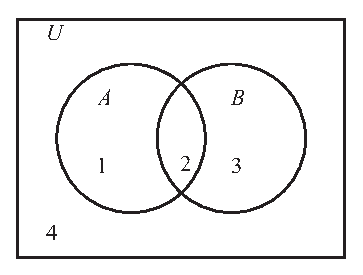
\includegraphics{figps-venn2.eps}
%\caption{Venn Diagram for Two Sets} \label{fig:venn2-prev}
\end{center}

\begin{enumerate}
\item In the standard Venn diagram for two sets, both  $\left( {A \cup B} \right)^c $  and  
$A^c  \cap B^c $ are represented by Region 4.	

\item Based on the Venn diagram, it appears that $\left( {A \cup B} \right)^c  = A^c  \cap B^c $.

\item An element  $x$  is not in $A \cup B$  means that  $x \notin A$  and  $x \notin B$.

\item An element  $x$  is in  $A^c $ means that  $x \notin A$.  In addition, $x \in B^c $  means that  
$x \notin B$.

\item An element  $x$  is in $A^c  \cap B^c $ means that   $x \in A^c $ and   $x \in B^c $.  So, $x \in A^c  \cap B^c $ means that   $x \notin A$ and   $x \notin B$.

\item The responses in (3) and (5) are equivalent.

\item As with the Venn diagram, this argument indicates that $\left( {A \cup B} \right)^c  = A^c  \cap B^c $.
\end{enumerate}
\hbreak


\newpage
\subsection*{Beginning Activity 2 (Proving that Statements Are Equivalent)}
\begin{enumerate}
\item 
\begin{tabular}[t]{| c | c | c || c | c | c | c | c | } \hline
$X$ & $Y$ & $Z$ &  $X \to Y$ & $Y \to Z$ & $X \to Z$ & $\left( {X \to Y} \right) \wedge \left( {Y \to Z} \right )$ & $\left[ {\left( {X \to Y} \right) \wedge \left( {Y \to Z} \right )} \right]$ \\ 
 & & & & & & & $\to \left( {X \to Z} \right)$ \\ \hline
T & T & T & T & T & T & T & T \\ \hline
T & T & F & T & F & F & F & T \\ \hline
T & F & T & F & T & T & F & T \\ \hline
T & F & F & F & T & F & F & T \\ \hline
F & T & T & T & T & T & T & T \\ \hline
F & T & F & T & F & T & F & T \\ \hline
F & F & T & T & T & T & T & T \\ \hline
F & F & F & T & T & T & T & T \\ \hline
\end{tabular}

\item The truth table in Part (1) shows that   
$\left[ {\left( {X \to Y} \right) \wedge \left( {Y \to Z} \right)} \right] \to \left( {X \to Z} \right)$  is a tautology.  (It is always true.)  This means that whenever we know that  $X \to Y$
  and that  $Y \to Z$, we can conclude that  $X \to Z$.

We are given that (1) $\left( {P \to Q} \right)$; (2) $\left( {Q \to R} \right)$; and  
(3) $\left( {R \to P} \right)$ are true.

\begin{enumerate}
\item So if the conditional statements in (1), (2), and (3) are true, then we know that  
$P \to Q$. We can use statements (2) and (3) to conclude that  $Q \to P$.  Therefore,  
$P \leftrightarrow Q$  is true.

\item We also know that  $Q \to R$, and we can use statements (3) and (1) to conclude that  
$R \to Q$.  Therefore,  $Q \leftrightarrow R$  is true.

\item We also know that  $R \to P$, and we can use statements (1) and (2) to conclude that  
$P \to R$.  Therefore,  $P \leftrightarrow R$  is true.
\end{enumerate}

\textbf{Note}:
When we have a list of three statements  $P$, $Q$,  and  $R$  such that  (1), (2), and (3) are true, we say that the three statements are \textbf{equivalent}.  This means that each of the statements in the list implies each of the other statements in the list.  

The purpose of this activity is to provide one way to prove that three (or more) statements are equivalent.  The basic idea is to prove a sequence of conditional statements (such as (1), (2), and (3)), so that there is an unbroken chain of conditional statements from each statement to every other statement.
\end{enumerate}
\hbreak

\end{document}
